\chapter{Input/Output}
\label{sc:io}

\section{NetCDF format}

%%%%%%%%%%%%%%%%%%%%%%%%%%
GCM input/output data are written in {\bf NetCDF} format
(Network Common Data Form). NetCDF is an interface used to store and access
geophysical data, and a library that provides an implementation of this
interface. The NetCDF library also defines a machine-independent format for
representing scientific data. 
Together, the interface, library and format support the creation, access and
sharing of scientific data. NetCDF was developed at the Unidata Program Center
in Boulder, Colorado. The freely available source can be obtained from
the Unidata website:
\begin{verbatim}
http://www.unidata.ucar.edu/software/netcdf
\end{verbatim}


%%%%%%%%%%%%%%%%%%%%%%%%%%

A data set in NetCDF format is a single file, as it is self-descriptive.

\subsection{NetCDF text representation: ncdump}

This utility is included in the NetCDF library.
It generates the CDL representation (text format of the file content) to the standard output
from the NetCDF file specified as input. 

\paragraph{Main options for the ncdump command}

\begin{center}
{\it ncdump diagfi.nc}
\end{center}

\noindent
dump contents of NetCDF file {\tt diagfi.nc} to standard output
(i.e. the screen).

\begin{center}
{\it ncdump -c diagfi.nc}
\end{center}

\noindent
Displays the {\bf coordinate} variable values (variables which are also
dimensions), as well as the declarations, variables and attribute values.
The values of the non-coordinate variable data are not displayed at
the output.

\begin{center}
{\it ncdump -h diagfi.nc}
\end{center}

\noindent
Shows only the informative header of the file, which is the declaration
of the dimensions, variables and attributes, but not the values of these
variables. The output is identical to that in option {\bf -c} except for
the fact that the coordinated variable values are not included.

\begin{center}
{\it ncdump -v var1,...,varn diagfi.nc}
\end{center}

\noindent
The output includes the specific variable values,
as well as all the dimensions, variables and attributes.
More that one variable can be specified in the list following this option.
The list must be a simple argument for the command, and must not contain any
spaces. If no variable is specified, the command displays all the values of
the variables in the file by default.  


\subsection{Graphic visualization of NetCDF files using GrAds}

GrAdS (The Grid Analysis and Display System) is a graphic software developed
by Brian Doty at the "Center for Ocean-Land-Atmosphere (COLA)".

One of its functions is to enable data stored in NetCDF format to be
visualized directly. In figure~\ref{fg:grads} for example, we can see the
GrADS visualization of the temperature data at a given moment.
%
\begin{figure}
\centering
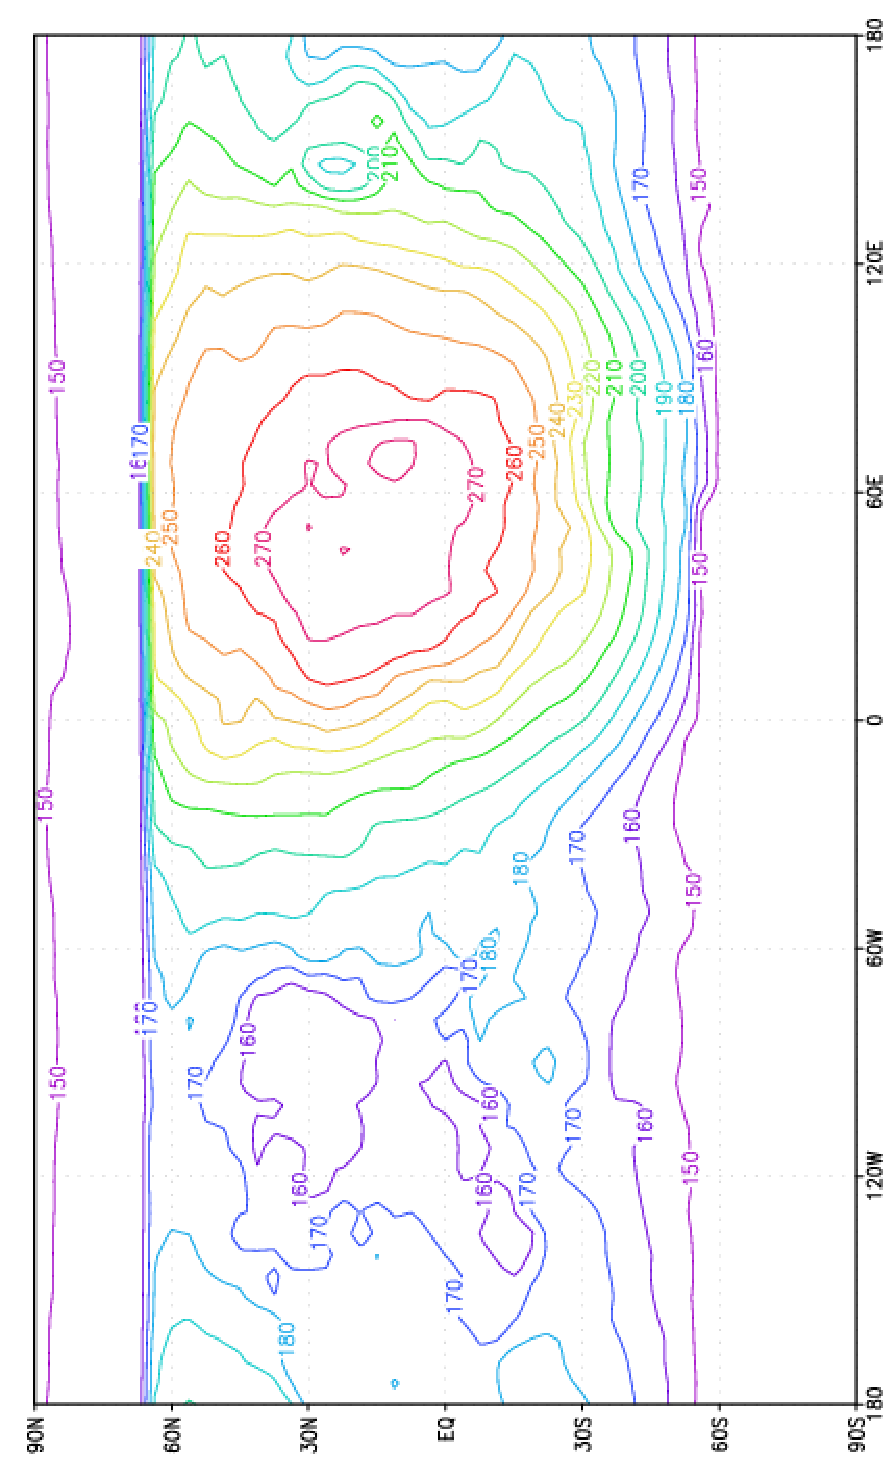
\includegraphics[width=0.5\textwidth,angle=270]{Fig/grads.pdf}
\caption{Example of temperature data at a given time using
GrADS visualization\label{fg:grads}}
\end{figure}
%
However, unlike NetCDF, GrADS only recognizes files where all the variables are stored on the same horizontal grid.
These variables can be in 1, 2, 3 or 4 dimensions (X,Y,Z and t).\\

GrADS can also be obtained from:
\begin{verbatim}
http://grads.iges.org/grads/
\end{verbatim}

\subsection{Graphic visualization of NetCDF files using Ferret}

Ferret may also be used to visualize the contents of NetCDF files. Download intruction and documentation are available from the official website:
\begin{verbatim}
https://ferret.pmel.noaa.gov/Ferret/
\end{verbatim} 

\section{Input and parameter files}

%{\bf \it Examples of initialization files can be found in directory
%\begin{verbatim}$PATH1/LMDZ.MARS/deftank \end{verbatim}}
\label{loc:entrees}

The (3D version of the) GCM requires
the input of two initialization files (in NetCDF format):\\
-{\bf start.nc}
contains the initial states of the dynamical variables.\\
-{\bf startfi.nc}
contains the initial states of the physical variables.\\
Note that collections of initial states can be retreived at:\\
\verb+http://www.lmd.jussieu.fr/~lmdz/planets/mars/starts+ \\
Extracting {\tt start.nc} and {\tt startfi.nc} from these archived
requires using program {\tt newstart}, as described in
section~\ref{sc:newstart}.\\

\noindent
To run, the GCM also requires the  four following
parameter files (ascii text files):\\
-{\bf run.def} the parameters of the dynamical part of the program,
and the temporal integration of the model.\\
-{\bf callphys.def} the parameters for calling the physical part.\\
-{\bf traceur.def} the names of the tracer to use.\\
-{\bf z2sig.def}
 the vertical distribution of the atmospheric layers.\\
Examples of these parameter files can be found in the
\verb+LMDZ.MARS/deftank+ directory.

\subsection{run.def}
\label{vb:run.def}
%%%%%%%%%%%%%%%%%%%%%%%%%%%%%%%%%%%%%%%%%%%%%%%%%%%%%%%
% run.def: les param sont lus dans dyn3d/defrun.F
%%%%%%%%%%%%%%%%%%%%%%%%%%%%%%%%%%%%%%%%%%%%%%%%%%%%%%%

A typical {\tt run.def} file is given as an example below.
The choice of variables to be set is simple (e.g.
 {\tt nday} number of modeled days to run),
while the others do not need to be changed for normal use.\\
The format of the {\tt run.def} file is quite straightforward
(and flexible): values given to parameters must be given as:
\begin{verbatim}
  parameter = value
\end{verbatim}
Any blank line or line beginning with symbol {\bf \#} is
a comment, and instruction lines may be written in any order.
Moreover, not specifying a parameter/value set (e.g. deleting it
or commenting it out) means you want the GCM to use a default built-in value.
Additionally, one may use a specific keyword {\bf INCLUDEDEF} to specify
another (text) file in which to also read values of parameters; e.g.:
\begin{verbatim}
INCLUDEDEF=callphys.def
\end{verbatim}


\noindent Here are some details about some of the parameters which may be
set in {\tt run.def}:
\begin{itemize}
\item {\bf day\_step}, the number of dynamical steps per day to use for
the time integration. This needs to be large enough for the model
to remain stable (this is related to the CFL stability criterion
which essentially depends on the horizontal resolution of the model).
On Mars, in theory, the GCM can run with
{\tt day\_step}=480 using the 64$\times$48 grid, but model stability
improves when this number is higher: {\tt day\_step}=960 is recommended
 when using the 64$\times$48 grid. According to the CFL criterion,
{\tt day\_step} should vary in proportion with the resolution: for example
{\tt day\_step}=480 using the 32$\times$24 horizontal resolution.
Note that {\tt day\_step} must also be divisible by {\tt iperiod}.

\item {\bf tetagdiv, tetagrot, tetatemp} control the dissipation intensity.
It is better to limit the dissipation intensity
(tetagdiv, tetagrot, tetatemp should not be too low).
However the model diverges if tetagdiv, tetagrot, tetatemp are too high,
especially if there is a lot of dust in the atmosphere. \\
Example used with nitergdiv=1 and  nitergrot=niterh=2 : \\
- using the 32$\times$24 grid tetagdiv=6000~s ; tetagrot=tetatemp=30000~s \\
- using the 64$\times$48 grid: tetagdiv=2500~s ; tetagrot=tetatemp=5000~s

\item {\bf idissip} is the time step used for the dissipation:
dissipation is computed and added every {\tt idissip} dynamical
time step. If {\tt idissip} is
too short, the model waste time in these calculations. But if idissip is too
long, the  dissipation will not be parametrized correctly and the  model will
be more likely to diverge. 
A check must be made, so that:
{\tt idissip}~$<$~{\tt tetagdiv}$\times${\tt daystep}/88775
(same rule for {\tt tetagrot} and {\tt tetatemp}).
This is tested automatically during the run.

\item {\bf iphysiq} is the time step used for the physics:
physical tendencies are computed every {\tt iphysiq} dynamical time step.
In practice, we
usually set the physical time step to be of the order of half an hour. 
We thus generally set {\tt iphysiq}= {\tt day\_step}/48

\end{itemize}

\noindent
{\it Example of run.def file: }
{\footnotesize
{\footnotesize
\begin{verbatim}

#------------------------------
# Parametres de controle du run
#------------------------------

# Nombre de jours d'integration
     nday=669

# nombre de pas par jour (multiple de iperiod) ( ici pour  dt = 1 min )
 day_step = 960

# periode pour le pas Matsuno (en pas)
  iperiod=5

# periode de sortie des variables de controle (en pas)
  iconser=120

# periode d'ecriture du fichier histoire (en jour)
    iecri=100

# periode de stockage fichier histmoy (en jour)
 periodav=60.

# periode de la dissipation (en pas)
  idissip=5

# choix de l'operateur de dissipation (star ou  non star )
 lstardis=.true.

# avec ou sans coordonnee hybrides
 hybrid=.true.

# nombre d'iterations de l'operateur de dissipation   gradiv
nitergdiv=1

# nombre d'iterations de l'operateur de dissipation  nxgradrot
nitergrot=2

# nombre d'iterations de l'operateur de dissipation  divgrad
   niterh=2

# temps de dissipation des plus petites long.d ondes pour u,v (gradiv)
 tetagdiv=10000.

# temps de dissipation des plus petites long.d ondes pour u,v(nxgradrot)
 tetagrot=10000.

# temps de dissipation des plus petites long.d ondes pour  h ( divgrad)
 tetatemp=10000.

# coefficient pour gamdissip
  coefdis=0.

# choix du shema d'integration temporelle (Matsuno ou Matsuno-leapfrog)
  purmats=.false.

# avec ou sans physique
   physic=.true.

# periode de la physique (en pas)
  iphysiq=20

# choix d'une grille reguliere
  grireg=.true.

# frequence (en pas) de l'ecriture du fichier diagfi
 ecritphy=1920

# longitude en degres du centre du zoom
   clon=63.

# latitude en degres du centre du zoom
   clat=0.

# facteur de grossissement du zoom,selon longitude
  grossismx=1.

# facteur de grossissement du zoom ,selon latitude
 grossismy=1.

#  Fonction  f(y)  hyperbolique  si = .true.  , sinon  sinusoidale
  fxyhypb=.false.

# extension en longitude  de la zone du zoom  ( fraction de la zone totale)
   dzoomx= 0.

# extension en latitude de la zone  du zoom  ( fraction de la zone totale)
   dzoomy=0.

#  raideur du zoom en  X
    taux=2.

#  raideur du zoom en  Y
    tauy=2.

#  Fonction  f(y) avec y = Sin(latit.) si = .TRUE. ,  Sinon  y = latit.
  ysinus= .false.

# Avec sponge layer
  callsponge  = .true.

# Sponge:  mode0(u=v=0), mode1(u=umoy,v=0), mode2(u=umoy,v=vmoy)
  mode_sponge= 2

# Sponge:  hauteur de sponge (km)
  hsponge= 90

# Sponge:  tetasponge (secondes)
  tetasponge = 50000

# some definitions for the physics, in file 'callphys.def'
INCLUDEDEF=callphys.def


\end{verbatim}
}

}
%%%%%%%%%%%%%%%%%%%%%%%%%%%%%%%%%%%%%%%%%%%%%%%%%%%%%%%


\subsection{callphys.def}
\label{sc:callphys.def}
%%%%%%%%%%%%%%%%%%%%%%%%%%%%%%%%%%%%%%%%%%%%%%%%%%%%%%%
% callphys.def: les param sont lus dans phymars/inifis.F
%%%%%%%%%%%%%%%%%%%%%%%%%%%%%%%%%%%%%%%%%%%%%%%%%%%%%%%
The {\tt callphys.def} file (along the same format
as the {\tt run.def} file) contains parameter/value sets
for the physics.\\

 
\noindent
{\it Example of callphys.def file: }
{\footnotesize
{\footnotesize
\begin{verbatim}

## Orbit / general options
## ~~~~~~~~~~~~~~~~~~~~~~~
# Run with or without tracer transport ?
tracer    = .true.
# Diurnal cycle ?  if diurnal=false, diurnally averaged solar heating
diurnal   = .true.
# Seasonal cycle ? if season=false, Ls stays constant, to value set in "start"
season    = .true.
# Tidally resonant orbit ? must have diurnal=false, correct rotation rate in newstart
tlocked   = .false.
# Tidal resonance ratio ? ratio T_orbit to T_rotation
nres      = 10
# Write some more output on the screen ?
lwrite    = .false.
# Save statistics in file "stats.nc" ?
callstats = .true.
# Test energy conservation of model physics ?
enertest  = .true.

## Radiative transfer options
## ~~~~~~~~~~~~~~~~~~~~~~~~~~
# call radiative transfer?
callrad    = .true.
# the rad. transfer is computed every "iradia" physical timestep
iradia     = 4
# call multilayer correlated-k radiative transfer ?
corrk      = .true.
# folder in which correlated-k data is stored ?
corrkdir   = CO2_H2Ovar
# call visible gaseous absorption in radiative transfer ?
callgasvis = .true.
# Include Rayleigh scattering in the visible ?
rayleigh   = .true.
# Characteristic planetary equilibrium (black body) temperature
# This is used only in the aerosol radiative transfer setup. (see aerave.F)
tplanet    = 215.
# Output spectral OLR in 1D/3D?
specOLR    = .false.
# Output global radiative balance in file 'rad_bal.out' - slow for 1D!!
meanOLR    = .true.
# Variable gas species: Radiatively active ?
varactive  = .true.
# Variable gas species: Fixed vertical distribution ?
varfixed   = .false.
# Variable gas species: Saturation percentage value at ground ?
satval     = 0.0

## Star type
## ~~~~~~~~~
startype = 1
# ~~~~~~~~~~~~~~~~~~~~~~~~~~~~~~~~~~~~~~~~~~~~~~~~~~~~~~~~~~
# The choices are:
#
#	startype = 1		Sol        (G2V-class main sequence)
#	startype = 2		Ad Leo     (M-class, synthetic)
#   startype = 3        GJ644
#   startype = 4        HD128167
# ~~~~~~~~~~~~~~~~~~~~~~~~~~~~~~~~~~~~~~~~~~~~~~~~~~~~~~~~~~~
# Stellar flux at 1 AU. Examples:
# 1366.0 W m-2		Sol today
# 1024.5 W m-2		Sol today x 0.75 = weak early Sun
# 18.462 W m-2		The feeble Gl581
# 19.960 W m-2		Gl581 with e=0.38 orbital average
Fat1AU = 1024.5

## Tracer and aerosol options
## ~~~~~~~~~~~~~~~~~~~~~~~~~~
# Gravitational sedimentation of tracers (KEEP FALSE FOR NOW) ?
sedimentation = .false.

## Other physics options
## ~~~~~~~~~~~~~~~~~~~~~
# call turbulent vertical diffusion ?
calldifv = .true.
# call convective adjustment ?
calladj  = .true.
# call thermal conduction in the soil ?
callsoil = .true.

#########################################
## extra specific options for Early Mars
#########################################

## Tracer and aerosol options
## ~~~~~~~~~~~~~~~~~~~~~~~~~~
# Fixed aerosol distributions?
aerofixed     = .false.
# Varying H2O cloud fraction?
CLFvarying    = .false.
# H2O cloud fraction?
CLFfixval     = 0.5
# number mixing ratio of CO2 ice particles
Nmix_co2      = 100000.
# number mixing ratio of water ice particles
Nmix_h2o      = 100000.

## Water options
## ~~~~~~~~~~~~~
# Model water cycle
water         = .true.
# Model water cloud formation
watercond     = .true.
# Model water precipitation (including coagulation etc.)
waterrain     = .true.
# WATER: Precipitation threshold (simple scheme only) ?
rainthreshold = 0.0011
# Include hydrology ?
hydrology     = .true.
# H2O snow (and ice) albedo ?
albedosnow    = 0.5
# Maximum sea ice thickness ?
maxicethick   = 0.05
# Freezing point of seawater (degrees C) ?
Tsaldiff      = 0.0

## CO2 options
## ~~~~~~~~~~~
# gas is non-ideal CO2 ?
nonideal      = .false.
# call CO2 condensation ?
co2cond       = .true.
# Set initial temperature profile to 1 K above CO2 condensation everywhere?
nearco2cond   = .false.

\end{verbatim}
}

}
%%%%%%%%%%%%%%%%%%%%%%%%%%%%%%%%%%%%%%%%%%%%%%%%%%%%%%%

\subsection{traceur.def}
\label{sc:traceur.def}
Tracers in input ({\tt start.nc} and {\tt startfi.nc}) and output
files ({\tt restart.nc} and {\tt restartfi.nc}) are stored using
individual tracer names (e.g. {\tt co2} for CO2 gas, {\tt h2o\_vap}
for water vapour, {\tt h2o\_ice} for water ice, ...).\\
The first line of the {\tt traceur.def} file (an ASCII file) must
contain the number of tracers to load and use (this number should
be the same as given to the {\tt -t} option of the {\tt makegcm}
script when the GCM was compiled), followed by the tracer names
(one per line). Note that if the corresponding tracers are not
found in input files {\tt start.nc} and {\tt startfi.nc}, then the
tracer is initialized to zero.\\


\noindent {\it Example of a traceur.def file}:
with CO2, dust distribution moments, (water ice) cloud condensation nuclei moments, water vapour and water ice tracers
{\footnotesize
\begin{verbatim}
7
co2
dust_number
dust_mass
ccn_number
ccn_mass
h2o_ice
h2o_vap
\end{verbatim}
}

\subsection{z2sig.def}
The {\tt Z2sig.def} file contains the pseudo-altitudes
(in km) at which the user wants to set the vertical levels.\\
Note that levels should be unevenly spread, with a higher resolution
near the surface in order to capture the rapid variations of variables
there. It is recommended to use the altitude levels as set in the
{\tt z2sig.def} file provided in the {\tt deftank} directory.\\


\noindent
{\it Example of  z2sig.def file
(this version for 49 layers between  0 and 300~km):}
{\footnotesize
\begin{verbatim}
10.00000     H: atmospheric scale height (km) (used as a reference only)
0.0040       Typical pseudo-altitude (m) for 1st layer (z=H*log(sigma))
0.018       ,, ,,  ,, ,, ,, ,,  ,, ,, ,,  2nd layer, etc...
0.0400
0.1000
0.228200
0.460400
0.907000
1.73630
3.19040
5.54010
8.97780
13.5138
18.9666
25.0626
31.5527
38.4369
45.4369
52.4369
\end{verbatim}

}

\subsection{Initialization files: start and startfi}

%
\begin{figure}[h]
\centering
\framebox[0.8\textwidth][c]{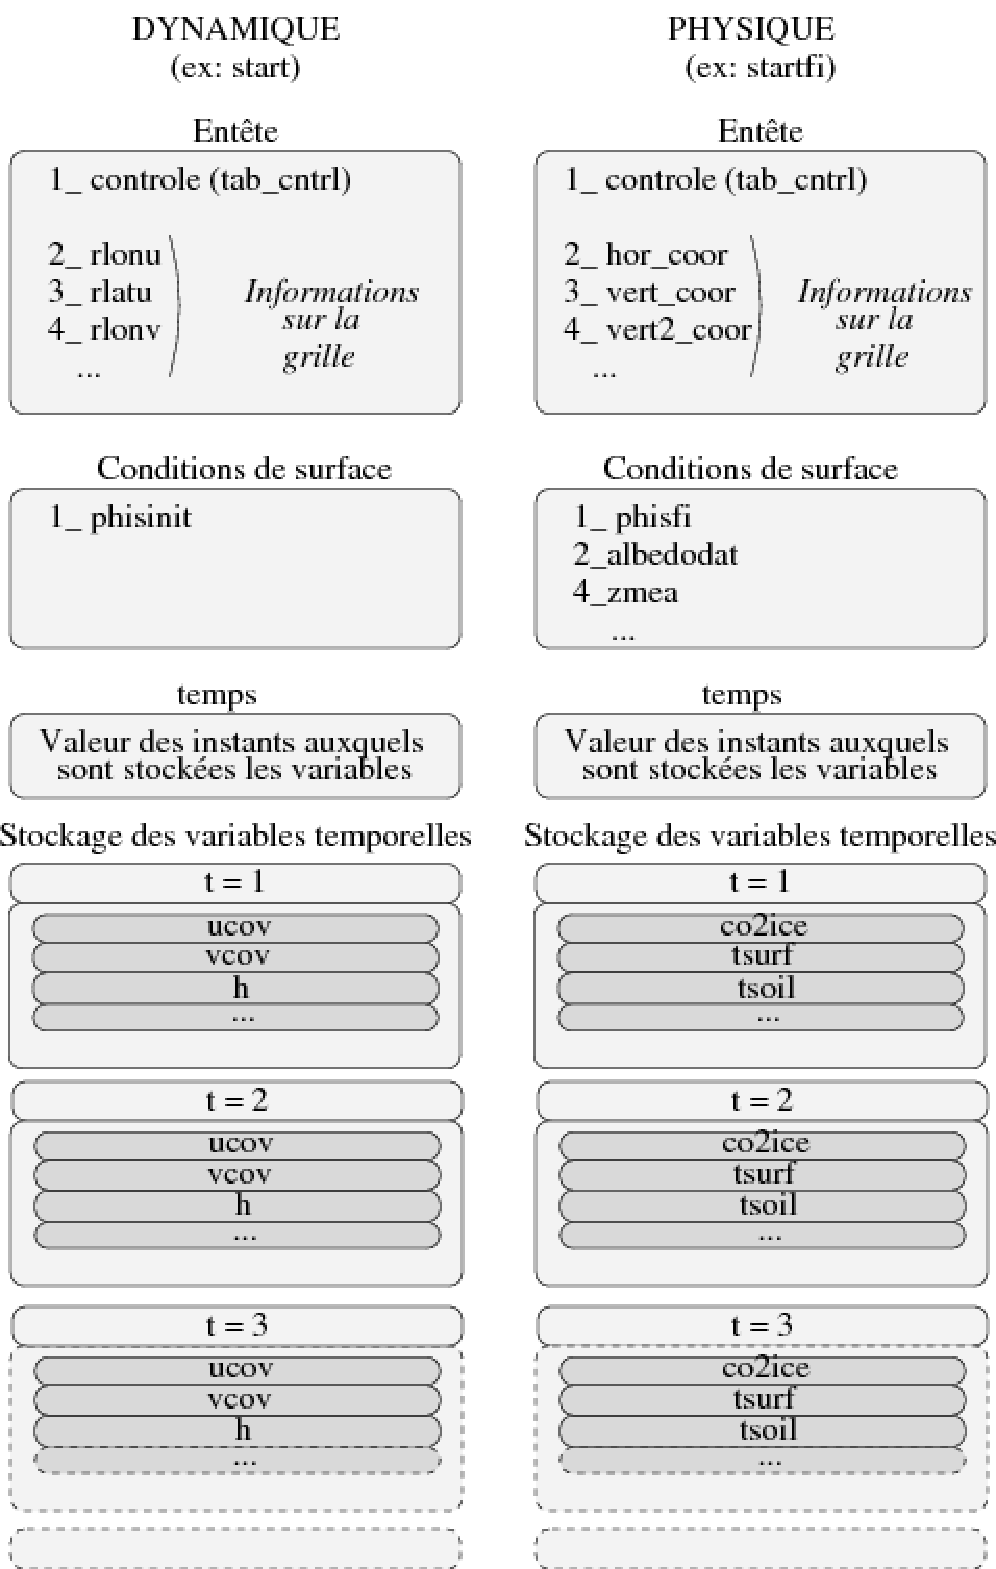
\includegraphics[width=0.7\textwidth]{Fig/netcdf.pdf}}
\caption{Organization of NetCDF files \label{fg:netcdf}}
\end{figure}
%
Files {\tt start.nc} and {\tt startfi.nc}, like all the NetCDF files of
the GCM,
are constructed on the same model (see NetCDF file composition,
figure~\ref{fg:netcdf}). They contain:\\
- a header with a ``control'' variable followed by a series of variables
defining the (physical and dynamical) grids \\
- a series of non temporal variables that give information about surface 
conditions on the planet.\\
- a ``time'' variable giving the values of the different instants at which 
the temporal variables are stored 
(a single time value (t=0) for start,
as it describes the dynamical initial states,
and no time values for startfi, as it describes only a physical state).\\

To dump (in text format) the contents of a {\tt start.nc} file using the
{\tt ncdump} command:\\

\noindent
{\it ncdump -h start.nc}\\
%%%%%%%%%%%%%%%%%%%%%%%%%%%%%%%%%%%%%%%%%%%%%%%%%%%%%%%
% List START
%%%%%%%%%%%%%%%%%%%%%%%%%%%%%%%%%%%%%%%%%%%%%%%%%%%%%%%
{\footnotesize
\begin{verbatim}
netcdf start {
dimensions:
        index = 100 ;
        rlonu = 33 ;
        latitude = 25 ;
        longitude = 33 ;
        rlatv = 24 ;
        altitude = 18 ;
        interlayer = 19 ;
        Time = UNLIMITED ; // (1 currently)
variables:
        float controle(index) ;
                controle:title = "Parametres de controle" ;
        float rlonu(rlonu) ;
                rlonu:title = "Longitudes des points U" ;
        float rlatu(latitude) ;
                rlatu:title = "Latitudes des points U" ;
        float rlonv(longitude) ;
                rlonv:title = "Longitudes des points V" ;
        float rlatv(rlatv) ;
                rlatv:title = "Latitudes des points V" ;
        float ap(interlayer) ;
                ap:title = "Coef A: hybrid pressure levels" ;
        float bp(interlayer) ;
                bp:title = "Coef B: hybrid sigma levels" ;
        float aps(altitude) ;
                aps:title = "Coef AS: hybrid pressure at midlayers" ;
        float bps(altitude) ;
                bps:title = "Coef BS: hybrid sigma at midlayers" ;
        float presnivs(altitude) ;
        float latitude(latitude) ;
                latitude:units = "degrees_north" ;
                latitude:long_name = "North latitude" ;
        float longitude(longitude) ;
                longitude:long_name = "East longitude" ;
                longitude:units = "degrees_east" ;
        float altitude(altitude) ;
                altitude:long_name = "pseudo-alt" ;
                altitude:units = "km" ;
                altitude:positive = "up" ;
        float cu(latitude, rlonu) ;
                cu:title = "Coefficient de passage pour U" ;
        float cv(rlatv, longitude) ;
                cv:title = "Coefficient de passage pour V" ;
        float aire(latitude, longitude) ;
                aire:title = "Aires de chaque maille" ;
        float phisinit(latitude, longitude) ;
                phisinit:title = "Geopotentiel au sol" ;
        float Time(Time) ;
                Time:title = "Temps de simulation" ;
                Time:units = "days since    1-01-01 00:00:00" ;
        float ucov(Time, altitude, latitude, rlonu) ;
                ucov:title = "Vitesse U" ;
        float vcov(Time, altitude, rlatv, longitude) ;
                vcov:title = "Vitesse V" ;
        float teta(Time, altitude, latitude, longitude) ;
                teta:title = "Temperature" ;
        float h2o_ice(Time, altitude, latitude, longitude) ;
                h2o_ice:title = "Traceur h2o_ice" ;
        float h2o_vap(Time, altitude, latitude, longitude) ;
                h2o_vap:title = "Traceur h2o_vap" ;
        float masse(Time, altitude, latitude, longitude) ;
                masse:title = "C est quoi ?" ;
        float ps(Time, latitude, longitude) ;
                ps:title = "Pression au sol" ;

// global attributes:
                :title = "Dynamic start file" ;
}
\end{verbatim}
}

%%%%%%%%%%%%%%%%%%%%%%%%%%%%%%%%%%%%%%%%%%%%%%%%%%%%%%%

\noindent
List of contents of a {\tt startfi.nc} file:\\

\noindent
{\it ncdump -h startfi.nc}\\
%%%%%%%%%%%%%%%%%%%%%%%%%%%%%%%%%%%%%%%%%%%%%%%%%%%%%%%
% List startfi
%%%%%%%%%%%%%%%%%%%%%%%%%%%%%%%%%%%%%%%%%%%%%%%%%%%%%%%
{\footnotesize
\begin{verbatim}
netcdf startfi {
dimensions:
        index = 100 ;
        physical_points = 738 ;
        subsurface_layers = 18 ;
        nlayer_plus_1 = 19 ;
        number_of_advected_fields = 3 ;
variables:
        float controle(index) ;
                controle:title = "Control parameters" ;
        float soildepth(subsurface_layers) ;
                soildepth:title = "Soil mid-layer depth" ;
        float longitude(physical_points) ;
                longitude:title = "Longitudes of physics grid" ;
        float latitude(physical_points) ;
                latitude:title = "Latitudes of physics grid" ;
        float area(physical_points) ;
                area:title = "Mesh area" ;
        float phisfi(physical_points) ;
                phisfi:title = "Geopotential at the surface" ;
        float albedodat(physical_points) ;
                albedodat:title = "Albedo of bare ground" ;
        float ZMEA(physical_points) ;
                ZMEA:title = "Relief: mean relief" ;
        float ZSTD(physical_points) ;
                ZSTD:title = "Relief: standard deviation" ;
        float ZSIG(physical_points) ;
                ZSIG:title = "Relief: sigma parameter" ;
        float ZGAM(physical_points) ;
                ZGAM:title = "Relief: gamma parameter" ;
        float ZTHE(physical_points) ;
                ZTHE:title = "Relief: theta parameter" ;
        float co2ice(physical_points) ;
                co2_ice:title = "CO2 ice cover" ;
        float inertiedat(subsurface_layers, physical_points) ;
                inertiedat:title = "Soil thermal inertia" ;
        float tsurf(physical_points) ;
                tsurf:title = "Surface temperature" ;
        float tsoil(subsurface_layers, physical_points) ;
                tsoil:title = "Soil temperature" ;
        float emis(physical_points) ;
                emis:title = "Surface emissivity" ;
        float q2(nlayer_plus_1, physical_points) ;
                q2:title = "pbl wind variance" ;
        float h2o_ice(physical_points) ;
                h2o_ice:title = "tracer on surface" ;

// global attributes:
                :title = "Physics start file" ;
}
\end{verbatim}
}

%%%%%%%%%%%%%%%%%%%%%%%%%%%%%%%%%%%%%%%%%%%%%%%%%%%%%%%



%%%%%%%%%%%%%%%%%%%%%%%%%%%%%%%%%%%%%%%%%%%%%%%%%%%%%%%
%    Description des start et startfi
%%%%%%%%%%%%%%%%%%%%%%%%%%%%%%%%%%%%%%%%%%%%%%%%%%%%%%%

\paragraph{Physical and dynamical headers}

There are two types of headers: one for the physical headers,
and one for the dynamical headers.
The headers always begin with a ``control' variable
(described below), that is allocated differently in the physical and
dynamical parts.
The other variables in the header concern the (physical and dynamical) grids.
They are the following:\\

\noindent
the horizontal coordinates\\
- {\bf rlonu}, {\bf rlatu}, {\bf rlonv}, {\bf rlatv} for the dynamical part,\\
- {\bf lati}, {\bf long} for the physical part,\\

\noindent
the coefficients for passing from the physical grid to the dynamical grid\\
- {\bf cu},{\bf cv} only in the dynamical header\\

\noindent
and finally, the grid box areas\\
- {\bf aire} for the dynamical part,\\
- {\bf area} for the physical part.\\

\paragraph{Surface conditions}

The surface conditions are mostly given in the physical NetCDF files by
variables:\\
- {\bf phisfi} for the initial state of surface geopotential,\\
- {\bf albedodat} for the bare ground albedo,\\
- {\bf inertiedat} for the surface thermal inertia,\\
- {\bf zmea}, {\bf zstd}, {\bf zsig}, {\bf zgam} and {\bf zthe} for
  the subgrid scale topography.\\

\noindent
For the dynamics:\\
- {\bf physinit} for the initial state of surface geopotential\\

\noindent
Remark: variables {\bf phisfi} and {\bf physinit} contain the same information
(surface geopotential), but {\bf phisfi} gives the geopotential values on the
physical grid, while {\bf physinit} give the values on the dynamical grid.\\

\paragraph{Physical and dynamical state variables}
To save disk space, the initialization files store the variables used by
the model, rather than the ``natural'' variables.\\

\noindent
For the dynamics:
\begin{description}
\item - {\bf ucov} and {\bf vcov} the covariant winds\\
These variables are linked to the ``natural'' winds by\\
\verb+ucov = cu * u+ and \verb+vcov = cv * v+
\item - {\bf teta} the potential temperature,\\
  or more precisely, the potential enthalpy linked to temperature {\bf T} by
  $\theta = T\dep{\frac{P}{Pref}}^{-K}$
\item - the tracers,
\item - {\bf ps} surface pressure.
\item - {\bf masse} the atmosphere mass in each grid box.
\end{description}

\noindent
``Vectorial'' variables {\bf ucov} and {\bf vcov} are stored on
``staggered'' grids u and v respectively (in the dynamics)
(see section \ref{fg:grid}).\\
Scalar variables {\bf h}, {\bf q} (tracers), {\bf ps}, {\bf masse} are stored
on the ``scalar'' grid of the dynamical part.\\

\noindent
For the physics:
\begin{description}
\item - {\bf co2ice} surface dry ice,
\item - {\bf tsurf} surface temperature,
\item - {\bf tsoil} temperatures at different layers under the surface,
\item - {\bf emis} surface emissivity,
\item - {\bf q2} wind variance,\\
or more precisely, the square root of the turbulent kinetic energy.
\item - the surface ``tracer'' budget
 (kg.m$^{-2}$),\\
\end{description}

\noindent
All these variables are stored on the ``physical'' grid
(see section \ref{fg:grid}).\\
%%%%%%%%%%%%%%%%%%%%%%%%%%%%%%%%%%%%%%%%%%%%%%%%%%%%%%%

\paragraph{The ``control'' array}

\indent
Both physical and dynamical headers of the GCM NetCDF files start with
a {\bf controle} variable. This variable is an array of 100 reals (the vector
called {\tt tab\_cntrl} in the program), which contains the program control
parameters. 
Parameters differ between the physical and dynamical sections, and examples
of both are listed below. The contents of table {\tt tab\_cntrl} can also
be checked with the command {\tt ncdump -ff -v controle}.\\

\noindent
{\bf The "control" array in the header of a dynamical NetCDF file:
start}
%%%%%%%%%%%%%%%%%%%%%%%%%%%%%%%%%%%%%%%%%%%%%%%%%%%%%%%
% tab_cntrl (dynamique) dans dyn3d/inimomo.F
%%%%%%%%%%%%%%%%%%%%%%%%%%%%%%%%%%%%%%%%%%%%%%%%%%%%%%%
{\footnotesize
\begin{verbatim}
       tab_cntrl(1)  = FLOAT(iim) ! number of nodes along longitude
       tab_cntrl(2)  = FLOAT(jjm) ! number of nodes along latitude
       tab_cntrl(3)  = FLOAT(llm) ! number of atmospheric layers
       tab_cntrl(4)  = FLOAT(idayref) ! initial day 
       tab_cntrl(5)  = rad   ! radius of the planet
       tab_cntrl(6)  = omeg  ! rotation of the planet (rad/s)
       tab_cntrl(7)  = g     ! gravity (m/s2) ~3.72 for Mars
       tab_cntrl(8)  = cpp 
       tab_cntrl(9) = kappa   ! = r/cp
       tab_cntrl(10) = daysec ! lenght of a sol (s) ~88775
       tab_cntrl(11) = dtvr   ! dynamical time step (s)
       tab_cntrl(12) = etot0  ! total energy
       tab_cntrl(13) = ptot0  ! total pressure
       tab_cntrl(14) = ztot0  ! total enstrophy
       tab_cntrl(15) = stot0  ! total enthalpy
       tab_cntrl(16) = ang0   ! total angular momentum
       tab_cntrl(17) = pa     
       tab_cntrl(18) = preff  ! reference pressure (Pa)
       tab_cntrl(19)  = clon  ! longitude of center of zoom
       tab_cntrl(20)  = clat  ! latitude of center of zoom
       tab_cntrl(21)  = grossismx ! zooming factor, along longitude
       tab_cntrl(22)  = grossismy ! zooming factor, along latitude

       tab_cntrl(24) = dzoomx ! extention (in longitude) of zoom
       tab_cntrl(25) = dzoomy ! extention (in latitude) of zoom

       tab_cntrl(27) = taux ! stiffness factor of zoom in longitude
       tab_cntrl(28) = tauy ! stiffness factor of zoom in latitude
\end{verbatim}
}

%%%%%%%%%%%%%%%%%%%%%%%%%%%%%%%%%%%%%%%%%%%%%%%%%%%%%%%

\noindent
{\bf The "controle" array in the header of a physical NetCDF file:
startfi.nc}
%%%%%%%%%%%%%%%%%%%%%%%%%%%%%%%%%%%%%%%%%%%%%%%%%%%%%%%
% tab_cntrl (physique) dans phymars/iniwritefi.F
%%%%%%%%%%%%%%%%%%%%%%%%%%%%%%%%%%%%%%%%%%%%%%%%%%%%%%%
{\footnotesize
\begin{verbatim}
c Informations on the physics grid
      tab_cntrl(1) = float(ngridmx)  ! number of nodes on physics grid
      tab_cntrl(2) = float(nlayermx) ! number of atmospheric layers
      tab_cntrl(3) = day_ini + int(time)         ! initial day 
      tab_cntrl(4) = time -int(time)            ! initiale time of day

c Informations about Mars, used by dynamics and physics
      tab_cntrl(5) = rad      ! radius of Mars (m) ~3397200
      tab_cntrl(6) = omeg     ! rotation rate (rad.s-1)
      tab_cntrl(7) = g        ! gravity (m.s-2) ~3.72
      tab_cntrl(8) = mugaz    ! Molar mass of the atmosphere (g.mol-1) ~43.49
      tab_cntrl(9) = rcp      !  = r/cp  ~0.256793 (=kappa dans dynamique)
      tab_cntrl(10) = daysec  ! length of a sol (s)  ~88775

      tab_cntrl(11) = phystep  ! time step in the physics
      tab_cntrl(12) = 0.
      tab_cntrl(13) = 0.

c Informations about Mars, only for physics
      tab_cntrl(14) = year_day  ! length of year (sols) ~668.6
      tab_cntrl(15) = periheli  ! min. Sun-Mars distance (Mkm) ~206.66
      tab_cntrl(16) = aphelie   ! max. SUn-Mars distance (Mkm) ~249.22
      tab_cntrl(17) = peri_day  ! date of perihelion (sols since N. spring)
      tab_cntrl(18) = obliquit  ! Obliquity of the planet (deg) ~23.98

c Boundary layer and turbulence
      tab_cntrl(19) = z0        ! surface roughness (m) ~0.01
      tab_cntrl(20) = lmixmin   ! mixing length ~100
      tab_cntrl(21) = emin_turb ! minimal energy ~1.e-8

c Optical properties of polar caps and ground emissivity
      tab_cntrl(22) = albedice(1)  ! Albedo of northern cap ~0.5
      tab_cntrl(23) = albedice(2)  ! Albedo of southern cap ~0.5
      tab_cntrl(24) = emisice(1)   ! Emissivity of northern cap ~0.95
      tab_cntrl(25) = emisice(2)   ! Emissivity of southern cap ~0.95
      tab_cntrl(26) = emissiv      ! Emissivity of martian soil ~.95
      tab_cntrl(31) = iceradius(1) ! mean scat radius of CO2 snow (north)
      tab_cntrl(32) = iceradius(2) ! mean scat radius of CO2 snow (south)
      tab_cntrl(33) = dtemisice(1) ! time scale for snow metamorphism (north)
      tab_cntrl(34) = dtemisice(2) ! time scale for snow metamorphism (south)

c dust aerosol properties
      tab_cntrl(27) = tauvis      ! mean visible optical depth

      tab_cntrl(28) = 0. 
      tab_cntrl(29) = 0.
      tab_cntrl(30) = 0.

! Soil properties:
      tab_cntrl(35) = volcapa ! soil volumetric heat capacity
\end{verbatim}
}

%%%%%%%%%%%%%%%%%%%%%%%%%%%%%%%%%%%%%%%%%%%%%%%%%%%%%%%
 
\newpage
\section{Output files}

\subsection{NetCDF restart files - restart.nc and restartfi.nc}
These files are of the exact same format as {\tt start.nc} and
{\tt startfi.nc}
%%%%%%%%%%%%%%%%%%%%%%%%%%%%%%%%%%%%%%%%%%%%%%%%%%%%%%%
% Description des fichiers de Sortie
%%%%%%%%%%%%%%%%%%%%%%%%%%%%%%%%%%%%%%%%%%%%%%%%%%%%%%%

\subsection{ NetCDF file - diagfi.nc}
NetCDF file {\tt diagfi.nc} stores the instantaneous physical variables
throughout the simulation at regular intervals
(set by the value of parameter {\tt ecritphy} in 
parameter file {\tt run.def}; note that {\tt ecritphy} should be a
multiple of {\tt iphysiq} as well as a divisor of {\tt day\_step}).

\noindent
{\bf Any variable from any sub-routine of the physics can be stored
by calling subroutine} {\tt writediagfi}.
Moreover, one may add a {\tt diagfi.def} file containing only the names
of variables to output (one per line) in the directory where the GCM is
run, in order to have only thoses listed outputed in the {\tt diagfi.nc}
file.\\

\noindent
Illustrative example of the contents of a {\tt diagfi.nc}
file (using ncdump):\\
\noindent
{\it ncdump -h diagfi.nc}\\
%%%%%%%%%%%%%%%%%%%%%%%%%%%%%%%%%%%%%%%%%%%%%%%%%%%%%%%
% List DIAGFI
%%%%%%%%%%%%%%%%%%%%%%%%%%%%%%%%%%%%%%%%%%%%%%%%%%%%%%%
% temporaire!!!
{\footnotesize
\begin{verbatim}
netcdf diagfi {
dimensions:
        Time = UNLIMITED ; // (12 currently)
        index = 100 ;
        rlonu = 65 ;
        latitude = 49 ;
        longitude = 65 ;
        rlatv = 48 ;
        interlayer = 26 ;
        altitude = 25 ;
        subsurface_layers = 18 ;
variables:
        float Time(Time) ;
                Time:long_name = "Time" ;
                Time:units = "days since 0000-00-0 00:00:00" ;
        float controle(index) ;
                controle:title = "Control parameters" ;
        float rlonu(rlonu) ;
                rlonu:title = "Longitudes at u nodes" ;
        float latitude(latitude) ;
                latitude:units = "degrees_north" ;
                latitude:long_name = "North latitude" ;
        float longitude(longitude) ;
                longitude:long_name = "East longitude" ;
                longitude:units = "degrees_east" ;
        float altitude(altitude) ;
                altitude:long_name = "pseudo-alt" ;
                altitude:units = "km" ;
                altitude:positive = "up" ;
        float rlatv(rlatv) ;
                rlatv:title = "Latitudes at v nodes" ;
        float aps(altitude) ;
                aps:title = "hybrid pressure at midlayers" ;
                aps:units = "Pa" ;
        float bps(altitude) ;
                bps:title = "hybrid sigma at midlayers" ;
                bps:units = "" ;
        float ap(interlayer) ;
                ap:title = "hybrid pressure at interlayers" ;
                ap:units = "Pa" ;
        float bp(interlayer) ;
                bp:title = "hybrid sigma at interlayers" ;
                bp:units = "" ;
        float soildepth(subsurface_layers) ;
                soildepth:long_name = "Soil mid-layer depth" ;
                soildepth:units = "m" ;
                soildepth:positive = "down" ;
        float cu(latitude, rlonu) ;
                cu:title = "Conversion coefficients cov <--> natural" ;
        float cv(rlatv, longitude) ;
                cv:title = "Conversion coefficients cov <--> natural" ;
        float aire(latitude, longitude) ;
                aire:title = "Mesh area" ;
        float phisinit(latitude, longitude) ;
                phisinit:title = "Geopotential at the surface" ;
        float emis(Time, latitude, longitude) ;
                emis:title = "Surface emissivity" ;
                emis:units = "w.m-1" ;
        float tsurf(Time, latitude, longitude) ;
                tsurf:title = "Surface temperature" ;
                tsurf:units = "K" ;
        float ps(Time, latitude, longitude) ;
                ps:title = "surface pressure" ;
                ps:units = "Pa" ;
        float co2ice(Time, latitude, longitude) ;
                co2ice:title = "co2 ice thickness" ;
                co2ice:units = "kg.m-2" ;
        float mtot(Time, latitude, longitude) ;
                mtot:title = "total mass of water vapor" ;
                mtot:units = "kg/m2" ;
        float icetot(Time, latitude, longitude) ;
                icetot:title = "total mass of water ice" ;
                icetot:units = "kg/m2" ;
        float tauTES(Time, latitude, longitude) ;
                tauTES:title = "tau abs 825 cm-1" ;
                tauTES:units = "" ;
        float h2o_ice_s(Time, latitude, longitude) ;
                h2o_ice_s:title = "surface h2o_ice" ;
                h2o_ice_s:units = "kg.m-2" ;
}
\end{verbatim}
}

%%%%%%%%%%%%%%%%%%%%%%%%%%%%%%%%%%%%%%%%%%%%%%%%%%%%%%%

\noindent
The structure of the file is thus as follows: 
\begin{description}
\item- the dimensions 
\item- variable ``time'' containing the time of the timestep stored in the
 file (in Martian days since the beginning of the run)
\item- variable ``control'' containing many parameters, as described above.
\item- from `` rhonu'' to 'phisinit'': a list of data describing the
 geometrical coordinates of the data file, plus the surface topography
\item- finally, all the 2D or 3D data stored in the run. 
\end{description}


\subsection{Stats files}

As an option ({\tt stats} must be set to {\tt .true.} in {\tt callphys.def}),
the model can accumulate any
variable from any subroutine of the physics by calling
subroutine \verb+ wstat+ 
\\ \\ 
\noindent
This save is performed at regular intervals 12 times a day.
An average of the daily evolutions over the whole run is calculated
(for example, for a 10 day run, the averages of the variable values at
0hTU, 2hTU, 4hTU,...24hTU are calculated), along with RMS standard
deviations of the variables. This ouput is given in 
file {\tt stats.nc}.\\


\noindent
Illustrative example of the contents of a {\tt stats.nc} file (using ncdump):\\
\noindent
{\it ncdump -h stats.nc}\\
{\footnotesize
\begin{verbatim}
netcdf stats {
dimensions:
        latitude = 49 ;
        longitude = 65 ;
        altitude = 25 ;
        llmp1 = 26 ;
        Time = UNLIMITED ; // (12 currently)
variables:
        float Time(Time) ;
                Time:title = "Time" ;
                Time:units = "days since 0000-00-0 00:00:00" ;
        float latitude(latitude) ;
                latitude:title = "latitude" ;
                latitude:units = "degrees_north" ;
        float longitude(longitude) ;
                longitude:title = "East longitude" ;
                longitude:units = "degrees_east" ;
        float altitude(altitude) ;
                altitude:long_name = "altitude" ;
                altitude:units = "km" ;
                altitude:positive = "up" ;
        float aps(altitude) ;
                aps:title = "hybrid pressure at midlayers" ;
                aps:units = "" ;
        float bps(altitude) ;
                bps:title = "hybrid sigma at midlayers" ;
                bps:units = "" ;
        float ps(Time, latitude, longitude) ;
                ps:title = "Surface pressure" ;
                ps:units = "Pa" ;
        float ps_sd(Time, latitude, longitude) ;
                ps_sd:title = "Surface pressure total standard deviation over th
e season" ;
                ps_sd:units = "Pa" ;
        float tsurf(Time, latitude, longitude) ;
                tsurf:title = "Surface temperature" ;
                tsurf:units = "K" ;
        float tsurf_sd(Time, latitude, longitude) ;
                tsurf_sd:title = "Surface temperature total standard deviation o
ver the season" ;
                tsurf_sd:units = "K" ;
        float co2ice(Time, latitude, longitude) ;
                co2ice:title = "CO2 ice cover" ;
                co2ice:units = "kg.m-2" ;
        float co2ice_sd(Time, latitude, longitude) ;
                co2ice_sd:title = "CO2 ice cover total standard deviation over t
he season" ;
                co2ice_sd:units = "kg.m-2" ;
        float fluxsurf_lw(Time, latitude, longitude) ;
                fluxsurf_lw:title = "Thermal IR radiative flux to surface" ;
                fluxsurf_lw:units = "W.m-2" ;
        float fluxsurf_lw_sd(Time, latitude, longitude) ;
                fluxsurf_lw_sd:title = "Thermal IR radiative flux to surface tot
al standard deviation over the season" ;
                fluxsurf_lw_sd:units = "W.m-2" ;
        float fluxsurf_sw(Time, latitude, longitude) ;
                fluxsurf_sw:title = "Solar radiative flux to surface" ;
                fluxsurf_sw:units = "W.m-2" ;
        float fluxsurf_sw_sd(Time, latitude, longitude) ;
                fluxsurf_sw_sd:title = "Solar radiative flux to surface total st
andard deviation over the season" ;
                fluxsurf_sw_sd:units = "W.m-2" ;
        float fluxtop_lw(Time, latitude, longitude) ;
                fluxtop_lw:title = "Thermal IR radiative flux to space" ;
                fluxtop_lw:units = "W.m-2" ;
        float fluxtop_lw_sd(Time, latitude, longitude) ;
                fluxtop_lw_sd:title = "Thermal IR radiative flux to space total 
standard deviation over the season" ;
                fluxtop_lw_sd:units = "W.m-2" ;
        float fluxtop_sw(Time, latitude, longitude) ;
                fluxtop_sw:title = "Solar radiative flux to space" ;
                fluxtop_sw:units = "W.m-2" ;
        float fluxtop_sw_sd(Time, latitude, longitude) ;
                fluxtop_sw_sd:title = "Solar radiative flux to space total stand
ard deviation over the season" ;
                fluxtop_sw_sd:units = "W.m-2" ;
        float dod(Time, latitude, longitude) ;
                dod:title = "Dust optical depth" ;
                dod:units = "" ;
        float dod_sd(Time, latitude, longitude) ;
                dod_sd:title = "Dust optical depth total standard deviation over
 the season" ;
                dod_sd:units = "" ;
        float temp(Time, altitude, latitude, longitude) ;
                temp:title = "Atmospheric temperature" ;
                temp:units = "K" ;
        float temp_sd(Time, altitude, latitude, longitude) ;
                temp_sd:title = "Atmospheric temperature total standard deviatio
n over the season" ;
                temp_sd:units = "K" ;
        float u(Time, altitude, latitude, longitude) ;
                u:title = "Zonal (East-West) wind" ;
                u:units = "m.s-1" ;
        float u_sd(Time, altitude, latitude, longitude) ;
                u_sd:title = "Zonal (East-West) wind total standard deviation ov
er the season" ;
                u_sd:units = "m.s-1" ;
        float v(Time, altitude, latitude, longitude) ;
                v:title = "Meridional (North-South) wind" ;
                v:units = "m.s-1" ;
        float v_sd(Time, altitude, latitude, longitude) ;
                v_sd:title = "Meridional (North-South) wind total standard devia
tion over the season" ;
                v_sd:units = "m.s-1" ;
        float w(Time, altitude, latitude, longitude) ;
                w:title = "Vertical (down-up) wind" ;
                w:units = "m.s-1" ;
        float w_sd(Time, altitude, latitude, longitude) ;
                w_sd:title = "Vertical (down-up) wind total standard deviation o
ver the season" ;
                w_sd:units = "m.s-1" ;
        float rho(Time, altitude, latitude, longitude) ;
                rho:title = "Atmospheric density" ;
                rho:units = "none" ;
        float rho_sd(Time, altitude, latitude, longitude) ;
                rho_sd:title = "Atmospheric density total standard deviation ove
r the season" ;
                rho_sd:units = "none" ;
        float q2(Time, altitude, latitude, longitude) ;
                q2:title = "Boundary layer eddy kinetic energy" ;
                q2:units = "m2.s-2" ;
        float q2_sd(Time, altitude, latitude, longitude) ;
                q2_sd:title = "Boundary layer eddy kinetic energy total standard
 deviation over the season" ;
                q2_sd:units = "m2.s-2" ;
        float vmr_h2ovapor(Time, altitude, latitude, longitude) ;
                vmr_h2ovapor:title = "H2O vapor volume mixing ratio" ;
                vmr_h2ovapor:units = "mol/mol" ;
        float vmr_h2ovapor_sd(Time, altitude, latitude, longitude) ;
                vmr_h2ovapor_sd:title = "H2O vapor volume mixing ratio total sta
ndard deviation over the season" ;
                vmr_h2ovapor_sd:units = "mol/mol" ;
        float vmr_h2oice(Time, altitude, latitude, longitude) ;
                vmr_h2oice:title = "H2O ice volume mixing ratio" ;
                vmr_h2oice:units = "mol/mol" ;
        float vmr_h2oice_sd(Time, altitude, latitude, longitude) ;
                vmr_h2oice_sd:title = "H2O ice volume mixing ratio total standar
d deviation over the season" ;
                vmr_h2oice_sd:units = "mol/mol" ;
        float mtot(Time, latitude, longitude) ;
                mtot:title = "total mass of water vapor" ;
                mtot:units = "kg/m2" ;
        float mtot_sd(Time, latitude, longitude) ;
                mtot_sd:title = "total mass of water vapor total standard deviat
ion over the season" ;
                mtot_sd:units = "kg/m2" ;
        float icetot(Time, latitude, longitude) ;
                icetot:title = "total mass of water ice" ;
                icetot:units = "kg/m2" ;
        float icetot_sd(Time, latitude, longitude) ;
                icetot_sd:title = "total mass of water ice total standard deviat
ion over the season" ;
                icetot_sd:units = "kg/m2" ;
}
\end{verbatim}
}


\noindent
The structure of the file is simillar to the {\tt diagfi.nc} file,
except that, as stated before, the average of variables are given for
12 times of the day and that RMS standard deviation are also provided.

